\documentclass[12pt]{article}
\usepackage{authblk}
\usepackage{graphicx} %used by PSL at least
\usepackage{amsmath}  %used by SHOC at least
\usepackage{natbib} %allows use of \citep{} and \citet{}
\bibliographystyle{amermeteorsoc}

\makeindex

\title{Design Document for the Simple Cloud-Resolving E3SM Atmosphere Model}
\author[1]{Peter Caldwell}
\author[2]{Andy Salinger}
\author[2]{Luca Bertagna}
\author[1]{Hassan Beydoun}
\author[1]{Peter Bogenschutz}
\author[2]{Andrew Bradley}
\author[5]{Conrad Clevenger}
\author[1]{Aaron Donahue}
\author[2]{Jim Foucar}
\author[1]{Chris Golaz}
\author[2]{Oksana Guba}
\author[2]{Ben Hillman}
\author[3]{Noel Keen}
\author[4]{Wuyin Lin}
\author[5]{Balwinder Singh}
\author[2]{Andrew Steyer}
\author[2]{Mark Taylor}
\author[1]{Chris Terai}
\author[6]{Paul Ullrich}
\date{\today}

\affil[1]{Lawrence Livermore National Lab, Livermore CA}
\affil[2]{Sandia National Laboratories, Albuquerque, NM}
\affil[3]{Lawrence Berkeley National Laboratory, Berkeley, CA}
\affil[4]{Brookhaven National Laboratory, Upton, NY}
\affil[5]{Pacific Northwest National Laboratory, Richland, WA}
\affil[6]{University of California, Davis, Davis, CA}

\begin{document}
\maketitle{}

\setcounter{tocdepth}{4}
\setcounter{secnumdepth}{4}
\tableofcontents

\newpage

\section{Overview}

Put description of model here as well as summary of what will/won't be in this document. Mention that there will be a separate user guide. Also, this doc isn't done until the list of authors is updated. Folks who joined after day 1 aren't included.

%INCLUDE SECTIONS FROM EACH PROCESS
%graphicspath forces latex to look for figures in each of the listed directories
\graphicspath{{control/}{physics/psl/}{dynamics/homme/}{physics/shoc/}{physics/p3/}{physics/rrtmgp/}}
%=-=-=-=-=-=-=-=-=-=-=-=-=-=-=-=-=-=-=-=-=-=-=-=-=-=-=-=-=-=-=-=-=-=-=-=-=-=-=-=
\section{Atmosphere Process Coupler}
%=-=-=-=-=-=-=-=-=-=-=-=-=-=-=-=-=-=-=-=-=-=-=-=-=-=-=-=-=-=-=-=-=-=-=-=-=-=-=-=
\subsection{Introduction}

This document details the development of the atmospheric model driver infrastructure for the Simplified Cloud Resolving E3SM Atmosphere Model (SCREAM) project.  The atmospheric driver for SCREAM will replace the Energy Exascale Earth System atmospheric model (EAM) driver.  The new Atmospheric Driver (AD) will incorporate many of the same features as the current EAM driver, but will simplify and clean up much of the code base and will be written in a modern C++ framework.

Taking advantage of the modern C++ architecture, the SCREAM--AD will introduce an atmospheric process class which will establish a simple and straightforward interface between the driver and individual atmospheric processes.  The passing of variables between processes will be greatly improved.  Model developers have often complained about the opaque structure of the current physics buffer (PBUF) approach particularly with the inability to properly audit which variables are being accessed and when.  In the SCREAM--AD, the PBUF will be replaced with an improved Field Manager (FM) class which will address many of these concerns.

This document is organized as follows: section \ref{sec:atmproc} explains how a process will be implemented within the atm\_process class. This will be followed by a description of how processes will be coupled together in section \ref{sec:proc_cpl}. Section \ref{sec:FM} will provide a description of how the Field Manager allows variables to be communicated between processes. Specification of runtime options and input/output will then be briefly described in \ref{sec:run_config} and \ref{sec:similarities}, respectively, before conclusions in section \ref{sec:concluding}.

%=-=-=-=-=-=-=-=-=-=-=-=-=-=-=-=-=-=-=-=-=-=-=-=-=-=-=-=-=-=-=-=-=-=-=-=-=-=-=-=
\subsection{Within an Atmospheric Process}
\label{sec:atmproc}
An atmospheric process is defined in SCREAM as any process that can change the model state.  This is in contrast to EAM which treats physics parameterizations and fluid dynamics very differently.  Handling fluid dynamics and physics parameterizations identically simplifies the AD and provides greater flexibility in the coupling infrastructure between processes (as described in section \ref{sec:proc_cpl}).  All atmospheric processes in SCREAM will be instances of an atmospheric process class, atm\_process.  The atmospheric process class will have three basic functions: initialization, run and finalization.  Developers of each parameterization are expected to supply implementations of the three functions customized for their scheme: 
\begin{itemize}
\item Initialization (called during the initialization stage of the AD) will:
	\begin{itemize}
	\item initialize all input/output (IO),
	\item register all process specific variables with the field manager (FM), see section \ref{sec:FM},
	\item allocate all local arrays and pointers. 
	\end{itemize}
\item Run (called each timestep during the run stage of the AD) will:
	\begin{itemize}
	\item retrieve variables from FM to be passed to the main process.
	\item conversion from the AD data structure to the data structure used within the parameterization of interest, if applicable.
	\item call the main process routine,
	\item postprocess output to save updated variables to the FM and to stage output for writing to NetCDF or ADIOS format
	\end{itemize}
\item Finalization (called during the finalization stage of the AD) will handle deallocation of all local arrays and pointers.
\end{itemize}

\subsubsection{Making Code Portable}
To make porting process representations to other models and running processes as standalone executables easy, the initialization, run, and finalize functions of each process will be broken into interface and process tasks. The interface code will grab needed input for the process from the FM and will ensure data is provided to the process calculation in the right format with the right units. It will then call the actual process code, which will do the actual calculation. After the process code completes, the interface code will convert output to the format required by the AD and/or FM. Because all dependencies on SCREAM-specific code are contained within the interface level, the process code will be easy to use outside of SCREAM. Tasks handled by the interface layer will range from simple tasks like obtaining density from the ideal gas law to complex tasks like switching to a different model grid, changing the geographic locations assigned to each processor, or even switching to a different set of processors to enable parallel execution over processes. Interface code will be distinguished from the actual process code by appending \emph{\_interface} to the appropriate file names. Developers can also append the suffix \emph{\_utils} to files to indicate these are helper files for that process.

\subsubsection{Basic SCREAM--AD Utilities}

{\bf It will be the responsibility of the process development team} to design the code for all of the steps mentioned so far in this section.  {\bf It will be the responsibility of the AD development team} to maintain the atm\_process class and to provide a checklist for new process development.  In addition, there will be a number of standard utilities developed in the SCREAM--AD that will assist process developers in bringing their processes into the SCREAM framework. The most powerful of these tools will be the field manager, which is the subject of section \ref{sec:FM}. The AD will also supply I/O routines, tools for accessing runtime options, energy and mass conservation checks, and timestepping schemes.

To promote consistency across the entire model, the AD will also provide a single location for all universal constants.  Developers will be encouraged to search this location for any constants that their specific process uses before adding new, process specific constants. If a constant isn't really universal (for example, parameters used only by a process-specific function) then they will be included in the \emph{$<$process\_name\_$>$\_utils} code. Similarly, there will be a C++ class for universal functions like linear regression or conversion from potential temperature to temperature.

%=-=-=-=-=-=-=-=-=-=-=-=-=-=-=-=-=-=-=-=-=-=-=-=-=-=-=-=-=-=-=-=-=-=-=-=-=-=-=-=
\subsection{Coupling Between Atmospheric Processes}
\label{sec:proc_cpl}

The initialization, run, and finalize methods for all processes included in the model will be called from top-level functions of the same name. The top-level initialization routine will also load the grid information for the SE dycore and for the physics mesh which depends on it. Our first implementation will use the existing Fortran code (with C++ wrappers) for domain initialization. To further simplify our initial version, we will use the dynamics grid decomposition for physics even though physics benefits from disbursing columns geographically while dynamics does best when all elements on a processor are neighbors. Future versions of SCREAM--AD will explore more sophisticated grid decomposition methods for physics, including use of a physics grid which is independent of dynamics (like \cite{herrington_physgrid}). Loading restart data will also be initially handled in the SCREAM--AD using C++ wrappers of Fortran routines from EAM. The top-level run routine will be called once per timestep, and will itself call the run interface function for each included process. These interface functions are themselves expected to call the actual process calculation as described above. It will also be responsible for ingesting inputdata, for writing output, and for interacting with the component coupler in order to obtain surface fluxes. At the finalization step the AD will call the finalization routine for each atmospheric process, deallocate the variables in the field manager (replacement for PBUF) and will deallocate any variables specific to the AD itself.

The top-level initialization, run, and finalize methods will initially handle processes one-at-a-time, but we will ensure these methods can be extended to operate on all processes simultaneously in the future. Because all processes are instances of the generic atm\_process class, it will be trivial to change process ordering or to add new processes. The SCREAM--AD will be designed to follow the process order given as a runtime option in an external YAML file (as described in section \ref{sec:run_config}). Because there are physical reasons for preferring certain process orders \cite{Donahue_param_order}, we envision ability to change ordering primarily as a tool for sensitivity testing and for ease of adding new processes. Attempts to use uninitialized variables will be caught by the FM.

If all processes are going to be treated identically, we can't have physics parameterizations return tendencies and dynamics return updated state. Our solution is to keep track of the state at the beginning of the timestep and a state after one or more processes have acted. All atmospheric processes will receive these two states as input. This allows processes to operate on the most recent state or to compute the tendencies from other processes (by differencing the initial and most-recent state) which can then be dribbled into the new process calculation over a series of substeps. Storing states rather than tendencies is better because converting from tendency to state can result in negative concentrations due to rounding errors which are avoided by insisting that all processes return non-negative values. 

For more advanced timestepping and splitting methods, the SCREAM--AD will back out tendencies from differences in state before and after parameterizations were called, then apply those tendencies to obtain a new state for the beginning of the next step.  

%=-=-=-=-=-=-=-=-=-=-=-=-=-=-=-=-=-=-=-=-=-=-=-=-=-=-=-=-=-=-=-=-=-=-=-=-=-=-=-=
\subsection{Passing Data Between Processes: The Field Manager}
\label{sec:FM}

Passing variables between processes is an important task for the AD. There are many options for how to do this, but most of them are problematic. For example, including all variables in a single derived datatype is unworkable because thousands of variables are passed between parameterizations and passing them all into/out of each parameterization would severely impact performance. Defining all variables required by multiple parameterizations in the AD-level "run" routine and passing just the variables needed between routines violates the "uniform input/output" requirement needed for each process to be a generic member of the atm\_process class. Including all variables in a single module loaded by all processes makes it too easy to access variables which aren't initialized yet. All of these methods are also problematic from the standpoint of writing restarts. Managing variables in a way which allows all variables needed for restarts to be written out in an automated loop has huge advantages. Ability to associate metadata with each variable is also very helpful. Not only does metadata allow for writing data to a more intelligible format than pure binary (e.g. a netCDF file), it also enables error checking that data dimensions and variable definitions are compatible.

The Physics BUFfer (PBUF) used in E3SMv1 provides a solution to these problems. It requires each parameterization that creates a field to give it the necessary data to allocate the field and assign it a name, as well as whether or not it will have to be written to a restart file.  Then any other process can request access to the same field through a pointer.  The use of pointers instead of full data arrays reduces the memory footprint of storing multiple copies of the same data.  The Field Manager (FM) in SCREAM will extend the PBUF from EAM, with all the functionality of the PBUF along with new features.  The essential differences between PBUF and the FM will be described in the next subsections.

\subsubsection{Specified intent of variables}
When an atmospheric process requests access to a variable in the FM it will also designate how the variable will be used, similar to intent IN, OUT, and IN/OUT in Fortran. This provides the FM with the ability to designate how a variable will be used when it is accessed.  

Designating how a variable is used will make it easier to track which atmospheric processes access the variable and where it is changed.  Each atmospheric process will have a set of two methods, \emph{required\_fields} and \emph{computed\_fields}, which will designate the list of fields needed by the process and changed by the process.  This will enable the field manager to provide a list of pointers to access those fields that includes that appropriate const correctness, depending on if we expect the field to be changed or not.  The field manager will have routines that create a schematic of all field managed variables, what routines use them and for what purpose.    By default, variables declared as \emph{required} will be controlled by declaring these variables as constants such that an error is raised if they are changed (const--correctness).  They will be further checked by comparing the time when the variable was last changed against the time when it was last expected to change.  For more robust variable audits, the field manager can keep a local copy of the entire set of field managed variables and compare with the same variables after each process is called to make sure only those variables that are intended to be changed are changed.  This would be a DEBUG flag compile option.


\subsubsection{Variables handled by the Field Manager}
Unlike EAM, which used derived datatypes to pass state and tendency information between physics parameterizations and PBUF to pass other variables, the FM will be used to pass \emph{all} variables.  This will eliminate the need to pass multiple structures between atmospheric processes.  Prognostic variables traditionally included in the EAM 'state' variable will continue to be treated differently. They will be given a special designation in FM which ensures they will be advected and prevents them from being designated output variables by parameterizations. Only allowing the AD layer to update these variables ensures that timestepping is handled centrally and important variables aren't updated by accident. If an atmospheric process needs to change a prognostic variable for internal calculations, it have to create a local copy of that variable for this purpose.

\subsubsection{AD data structure}
All fields stored in the FM will share a common data structure for consistency.  Given that most of the atmospheric processes in SCREAM use the physics domain the initial implementation of the FM will use the physics data structure on the physics map as the standard universal data structure.  This means that atmospheric processes that use a different data  or a different domain decomposition will need to map the FM managed variable to a local variable in the appropriate data structure in their interface layer.  For example, the dynamics interface will have to map data from the physics structure to the dynamics structure before calling the main dynamics routine and will need to map the output from dynamics back to the physics data structure before returning control to the AD.   This is what is currently done in E3SM via the \emph{pd\_coupling} and \emph{dp\_coupling} routines respectively.  The FM will have a set of mapping tools specifically designed to efficiently map between different data structures.

\subsubsection{Vectorization}
Every process which requests a field will include an optional input that specifies the length of vectorization, $N$, the process wants to use for that specific field.  If the optional input is not exercised than the assumption will be $N=1$, no vectorization.  The FM will then make sure the allocation for that field can accommodate all the requested vector lengths.


%=-=-=-=-=-=-=-=-=-=-=-=-=-=-=-=-=-=-=-=-=-=-=-=-=-=-=-=-=-=-=-=-=-=-=-=-=-=-=-=
\subsection{Specifying Runtime Options}
\label{sec:run_config}

Runtime options are a powerful tool from EAM that will be adopted in SCREAM.  In EAM, there are two sets of runtime options, those controlled by XML (e.g. env\_run.xml) and those controlled by namelist (see user\_nl\_cam).  Currently, the runtime options controlled by XML are related to CIME and involve global run settings such as run length, timestep, coupling frequency, run type, etc.  Model specific runtime options are handled by namelist.  The C++ coding language does not have an equivalent to the Fortran namelist parser, so a task of developing the SCREAM--AD is to design a user--interface in the C++ architecture.  The SCREAM--AD will adopt a YAML interface for handling runtime options.  

The combination of treating all processes as objects of the same class and using YAML to parse runtime options provides the flexibility to have the coupling mechanism between atmospheric processes be a runtime option.  Similarly, defining the process order will be straightforward using this interface.  

%=-=-=-=-=-=-=-=-=-=-=-=-=-=-=-=-=-=-=-=-=-=-=-=-=-=-=-=-=-=-=-=-=-=-=-=-=-=-=-=
\subsection{Input/Output}
\label{sec:similarities}

In its initial implementation, SCREAM--AD will adopt PIO2 for input and output. Because PIO2 supports ADIOS, this will allow us to take advantage of ADIOS' ability to write output to many local files rather than enduring the large communication costs needed to write to a single file at very high core counts.  Although PIO2 is written in C++, the F90 code layer needed to actually use it is complicated. Thus our initial version of SCREAM will call EAM's F90 I/O routines using C-to-Fortran wrappers.  These include the $addfld$, $outfld$, $add\_default$ and $whist$ routines.  Future versions of the AD will address rewriting the input/output routines in C++.  Because all variables handled by the FM will use the same data structure format, it will be easier to write output for any variable.  Like EAM, it will be possible to write out a variable's state at any point within a timestep even though most output will be sampled at the end of a timestep.  It will be possible to write restart files at any frequency, for example hourly, daily or monthly.  There will be a change to the standard naming convention used for scream based output, the current filename convention of RUNNAME.cam.hX.DATE.nc will be replaced with the more informative RUNNAME.{\bf scream.TYPE}.DATE.nc.  Where TYPE will be the frequency of output, e.g. daily, monthly, yearly, etc.

SCREAM--AD will be built using the same external libraries as CIME and as such will have access to all of the standard CIME tools including the \emph{perf\_mod} package of performance metrics.  Phase 1 of the SCREAM--AD will use a C++ wrapper to call the set of performance Fortran routines.  Taking advantage of the generalized ``atmospheric process'' object class, the placement of performance timer will be automatic for the initialization, running and finalization of all atmospheric processes.  This will be enforced by hard--coding the call to the performance timers inside the atmospheric process class.  There will also be the option to include extra timer flags to be called within a specific atmospheric process.

%=-=-=-=-=-=-=-=-=-=-=-=-=-=-=-=-=-=-=-=-=-=-=-=-=-=-=-=-=-=-=-=-=-=-=-=-=-=-=-=
\subsection{Concluding Remarks}
\label{sec:concluding}

The list of utilities described here is not an exhaustive list, but it represents the set of tasks and goals we believe are required to produce a working model in the three--year timeframe of the SCREAM project.  There are very likely other functions and utilities that will arise over the course of the project.  As such, the SCREAM--AD development process will be flexible and prepared to tackle any new issues as they come.  For example, when the new component coupler becomes available we anticipate devoting a major amount of resources towards incorporating this into the SCREAM--AD interface.


%=-=-=-=-=-=-=-=-=-=-=-=-=-=-=-=-=-=-=-=-=-=-=-=-=-=-=-=-=-=-=-=-=-=-=-=-=-=-=-=
%=-=-=-=-=-=-=-=-=-=-=-=-=-=-=-=-=-=-=-=-=-=-=-=-=-=-=-=-=-=-=-=-=-=-=-=-=-=-=-=
%=-=-=-=-=-=-=-=-=-=-=-=-=-=-=-=-=-=-=-=-=-=-=-=-=-=-=-=-=-=-=-=-=-=-=-=-=-=-=-=
%=-=-=-=-=-=-=-=-=-=-=-=-=-=-=-=-=-=-=-=-=-=-=-=-=-=-=-=-=-=-=-=-=-=-=-=-=-=-=-=
%=-=-=-=-=-=-=-=-=-=-=-=-=-=-=-=-=-=-=-=-=-=-=-=-=-=-=-=-=-=-=-=-=-=-=-=-=-=-=-=
%=-=-=-=-=-=-=-=-=-=-=-=-=-=-=-=-=-=-=-=-=-=-=-=-=-=-=-=-=-=-=-=-=-=-=-=-=-=-=-=
%=-=-=-=-=-=-=-=-=-=-=-=-=-=-=-=-=-=-=-=-=-=-=-=-=-=-=-=-=-=-=-=-=-=-=-=-=-=-=-=
%=-=-=-=-=-=-=-=-=-=-=-=-=-=-=-=-=-=-=-=-=-=-=-=-=-=-=-=-=-=-=-=-=-=-=-=-=-=-=-=



\section{Nonhydrostatic Spectral Element Dycore}

\subsection{Theory}

Put explanation of continuous equations here.

\subsection{Numerical Methods}

Describe the numerical methods used to discretize the equations here.

\subsection{Computational Implementation}

Describe the strategies used (if any) to ensure good computational performance.

\subsection{Verification}

Describe testing strategy

\section{Simplified Higher-Order Closure (SHOC)}

\subsection{Introduction}

Simplified Higher Order Closure \citep[SHOC;][]{Bogenschutz_Krueger13} is a parameterization of subgrid-scale (SGS) clouds and turbulence.  It is formulated to parameterize SGS shallow cumulus, stratiform cloud, and boundary layer turbulence in models that can either resolve deep convection or has an existing deep convection parameterization.  SHOC is an assumed-PDF based parameterization and uses a double Gaussian PDF to diagnose cloud fraction, cloud water, and higher-order turbulence moments.  SHOC is only a liquid cloud parameterization, thus it is assumed that any model SHOC is implemented in can treat the ice cloud phase. 

Table~\ref{table:prognostic} describes the SHOC prognostic variables and their nomenclature to be used throughout this document.  

\begin{table}[b]
\caption{Prognostic Variables in SHOC}
\centering
\begin{tabular}{c c c}
\hline\hline
variable & description & units \\
\hline
$\theta_{l}$ & Liquid water potential temperature & K \\
$q_{t}$ & Total water mixing ratio (vapor + cloud liquid) & kg/kg \\
$e$ & Turbulent kinetic energy & m$^2$/s$^2$ \\
$u$ & Zonal wind component & m/s \\
$v$ & Meridional wind component & m/s \\
$c$ & Tracer constituent & varies \\
\hline
\end{tabular}
\label{table:prognostic}
\end{table}

The liquid water potential temperature, $\theta_{l}$, is defined as:
%
\begin{equation}
  \theta_{l} \approx \theta - \frac{L_{v}}{c_{pd}}q_{l}
  \label{thetal}
\end{equation}
%
where $\theta$ is potential temperature, $L_{v}$ is the latent heat of vaporization, $c_{pd}$ the specific heat of dry air at constant pressure, $q_{l}$ the liquid water mixing ratio.  The turbulent kinetic energy ($\overline{e}$) is defined as
%
\begin{equation}
  \overline{e} = 0.5(\overline{u^{'2}}+\overline{v^{'2}}+\overline{w^{'2}}) , 
  \label{tke}
\end{equation}  
%
where $\overline{u^{'2}}$, $\overline{v^{'2}}$, and $\overline{w^{'2}}$ represent the SGS zonal, meridional, and vertical wind variances, respectively.  

In the SHOC parameterization, all prognostic variables are defined vertically at the mid-point of the grid box.  

Table~\ref{table:diagnostic} describes key diagnostic variables used throughout the SHOC parameterization, and their respective locations on the vertical grid.  Note that many diagnostic variables are defined at the interfaces of the grid box.  This is because many diagnostic variables are the result of centered vertical differences of the prognostic variables.  

\begin{table}[ht]
\caption{Key Diagnostic Variables in SHOC.  M in the location column indicates that the variable is located vertically in the mid-point of the grid box, while I indicates that the variable is located at the grid interfaces.}
\centering
\begin{tabular}{c c c c}
\hline\hline
variable & description & units & location \\
\hline
$L$ & Turbulent Length Scale & m & M \\
$\overline{\theta_{l}^{'2}}$ & Temperature variance & K$^2$ & I \\
$\overline{q_{t}^{'2}}$ & Moisture variance & kg$^2$/kg$^2$ & I \\
$\overline{w^{'2}}$ & Vertical velocity variance & m$^2$/s$^2$ & M \\
$\overline{w^{'}\theta_{l}^{'}}$ & Vertical temperature flux & K m/s & I \\
$\overline{w^{'}q_{t}^{'}}$ & Vertical moisture flux & m/s kg/kg & I \\
$\overline{q_{t}^{'}\theta_{l}^{'}}$ & Temperature and moisture covariance & K kg/kg & I \\
$\overline{w^{'3}}$ & Third moment of vertical velocity &  m$^3$/s$^3$ & I \\
$\overline{w^{'}\theta_{v}^{'}}$ & Buoyancy flux & K m/s & M \\
$K_{m}$ & Eddy diffusivity for momentum & m$^2$/s & M \\
$K_{h}$ & Eddy diffusivity for heat & m$^2$/s & M \\
\hline
\end{tabular}
\label{table:diagnostic}
\end{table}  

The code for SHOC breaks down each process into a separate subroutine.  Briefly, the order of operations of SHOC is described below.  Each process is then expanded upon with its own section.

SHOC order of operations:
\begin{enumerate}
  \item \textbf{Diagnose Turbulence Length Scale} (section~\ref{turb_scale}): The length scale represents the size of unresolved large eddies in a column.  This is needed to close the TKE equation and to diagnose several second order moments.
  \item \textbf{Solve the Turbulence Kinetic Energy Equation} (section~\ref{tke_equation}): Advance the TKE equation (due to shear production, buoyant production, and dissipation processes) one time step.  Note that advection of TKE is performed by the host model, while turbulent transport of TKE is done by SHOC turbulence diffusion.    
  \item \textbf{Perform Turbulence Diffusion} (section~\ref{turb_diffusion}): Using eddy coefficients derived from TKE, advance $\overline{u}$, $\overline{v}$, $\overline{\theta_{l}}$, $\overline{q_{t}}$ , $\overline{e}$, and any tracers ($\overline{c}$) one time step using an implicit diffusion solver.  
  \item \textbf{Diagnose the Second Order Moments} (section~\ref{diag_second}): Diagnose $\overline{q_{t}^{'2}}$, $\overline{\theta_{l}^{'2}}$, $\overline{q_{t}^{'}\theta_{l}^{'}}$, $\overline{w^{'2}}$, $\overline{w^{'}\theta_{l}^{'}}$, and $\overline{w^{'}q_{t}^{'}}$.  These are the second order moments needed to close the assumed PDF.
  \item \textbf{Diagnose the Third Order Moment} (section~\ref{diag_third}):  Diagnose the third moment of vertical velocity ($\overline{w^{'3}}$), needed to parameterize vertical velocity skewness in the assumed PDF
  \item \textbf{Compute Assumed PDF} (section~\ref{assumed_pdf}): Use the Assumed PDF to compute SGS cloud water, cloud fraction, and the buoyancy flux ($\overline{w^{'}\theta_{v}^{'}}$).
\end{enumerate}

In SHOC the order of operations is chosen deliberately so that the prognostic variables are updated first and the clouds are diagnosed last.  This is to prevent supersaturation from occurring when SHOC is complete, to avoid any potential conflicts with a microphysics scheme which may be called in the host model. 

%%%%%%%%%%%%%%%%%%%%%%%%%%%%%%%%%%%%%%%%%%%%%%%%%%%%%%%%%%%%%%%%%%%%%
%%%%%%%%%%%%%%%%%%%%%%%%%%%%%%%%%%%%%%%%%%%%%%%%%%%%%%%%%%%%%%%%%%%%%
%%%%%%%% TURBULENCE LENGTH SCALE
\subsection{Turbulence Length Scale}
\label{turb_scale}

The empirical formulation is based on the finding that the turbulent length scale is highly correlated with the distance from the wall, strength of the turbulence, boundary layer depth, and local thermal stability (Bogenschutz et al. 2010).  Within the turbulent boundary layer, the length scale definition is set equal to an asymptotic shape, similar to that of \cite{Blackadar_62}.  However it is weighted more strongly by the strength of the turbulence.  This reflects the behavior that as the grid size increases, the SGS TKE increases and so does the mixing length.  The effects of thermal stability are also included to reduce the length scale where the local stability is large.  

The formulation in (\ref{thelength}) is empirically determined from LES data and essentially represents a geometric average between the strength of the SGS TKE (as suggested by Texieria et al. 2004) and an asymptote length scale, with a contribution due to stability effects.  The geometric average assures that in close proximity to the surface, the length scale will be small.  
%
\begin{equation}
  L=\sqrt[]{8\left[\frac{1}{\tau\sqrt[]{e}kz}+\frac{1}{\tau\sqrt[]{e}L_{\infty}}+0.01\delta\frac{N^{2}}{\overline{e}}\right]^{-1}}
  \label{thelength}
\end{equation}

Above, $k$ is the von Karman constant.  $L_{\infty}$ is the asymptotic value of the length scale as defined in Blackadar (1962) as
%
 \begin{equation}
  L_{\infty}=0.1\frac{\int_{0}^{\infty}\overline{e}^{1/2}z dz}{\int_{0}^{\infty} \overline{e}^{1/2} dz}. 
  \end{equation}
 %
   In equation~\ref{thelength} $\delta$ is defined as:
\[
\delta = \left\{ 
\begin{array}{l l}
  1 & \quad \text{if} \quad N^{2} > 0 \\
  0 & \quad \text{if} \quad N^{2} \le 0 \\
\end{array} \right.
\]     
%
where $N^{2}$ is the moist Brunt Vaisala Frequency.  In SHOC $N^{2}$ is defined as:
%
\begin{equation}
  N^{2} = \frac{g}{\overline{\theta_{v}}}\frac{\partial{\overline{\theta_{v}}}}{\partial{z}}
  \label{brunt}
\end{equation}
%
where $\theta_{v}$ is the virtual potential temperature defined as:
%
\begin{equation}
  \theta_{v}=\theta(1 + 0.61q_{v} - q_{l}) , 
  \label{thetav}
\end{equation}
%
where $q_{v}$ is the water vapor mixing ratio. 
%
Finally, $\tau$ in equation~\ref{thelength} represents the eddy turnover timescale and is defined as
%
\begin{equation}
  \tau = \frac{D_{b}}{w_{*}},
  \label{conv_scale}
\end{equation} 

where $D_{b}$ is the boundary layer depth and is computed according to that of Holtslag and Boville (1993).  $w_{*}$ represents the convective velocity scale, integrated from the surface to the height of the boundary layer depth, and is defined as:
%
\begin{equation}
  w_{*}^{3}=2.5\frac{g}{\overline{\theta_{v}}} \int_{0}^{z_{D_{b}}} \overline{w^{'}\theta_{v}^{'}} dz .   
  \label{wstar_pbl}
\end{equation}

In the event that $w_{*}^{3} < 0$, which is indicative of a stable boundary layer, then $\tau$ is set to a default value of 100 s.  

%%%%%%%%%%%%%%%%%%%%%%%%%%%%%%%%%%%%%%%%%%%%%%%%%%%%%%%%%%%%%%%%%%%%%
%%%%%%%%%%%%%%%%%%%%%%%%%%%%%%%%%%%%%%%%%%%%%%%%%%%%%%%%%%%%%%%%%%%%%
%%%%%%%% TURBULENT KINETIC ENERGY
\subsection{Turbulent Kinetic Energy Equation}
\label{tke_equation}

In SHOC, the turbulent kinetic energy (TKE) equation to be solved is given by:
%
\begin{equation}
  \frac{\partial{\overline{e}}}{\partial{t}}=\underbrace{-\overline{u_{j}}\frac{\partial{\overline{e}}}{\partial{x_{j}}}}_\text{advection}+\underbrace{\frac{g}{\overline{\theta_{v}}}\left(\overline{w^{'}\theta_{v}^{'}}\right)}_\text{buoyant production}-\underbrace{P_{s}}_\text{shear production}-\underbrace{\frac{\partial{\overline{w^{'}e}}}{\partial{z}}}_\text{turbulent transport}-\underbrace{C_{ee}\frac{\overline{e}^{3/2}}{L}}_\text{dissipation} .  
  \label{sgstke}
\end{equation}

The first term on the RHS of equation~\ref{sgstke} is advection, which is performed by the host model (i.e. SCREAM dynamics) and not SHOC.  

The second term is the buoyant production of TKE.  The buoyancy flux term ($\overline{w^{'}\theta_{v}^{'}}$) is closed by integrating over the assumed PDF (see section~\ref{assumed_pdf}) using equation~\ref{buoyancy}.  Thus, $\overline{w^{'}\theta_{v}^{'}}$ from the previous SHOC time step is used to close this term.  

The shear production term is computed according to \cite{bretherton2009_moist}:
%
\begin{equation}
  -P_{s}= -\overline{w^{'}u^{'}}\frac{\partial{\overline{u}}}{\partial{z}}-\overline{w^{'}v^{'}}\frac{\partial{\overline{v}}}{\partial{z}} = K_{M}S^{2} , 
  \label{shearprod}
\end{equation}
%
where
\begin{equation}
  S^{2} = \left(\frac{\partial{\overline{u}}}{\partial{z}}\right)^2+\left(\frac{\partial{\overline{v}}}{\partial{z}}\right)^2 . 
  \label{tke_Sterm}
\end{equation}
%
Since $\overline{u}$ and $\overline{v}$ are located vertically in the mid-points, $S^{2}$ is computed on the interface grid, then interpolated onto the mid-point grid.  After the shear production term is calculated on the interface grid, it is interpolated to the mid-point grid to be consistent with the location of $\overline{e}$. 

The boundary surface value of $K_{M}S^{2}$ is set to zero as the boundary fluxes for TKE are applied in the diffusion solver.  

The fourth term on the RHS of equation~\ref{sgstke} represents the turbulent transport of TKE.  This term is computed in the turbulent diffusion (section~\ref{turb_diffusion}) of SHOC.  

The last term on the RHS of equation~\ref{sgstke} represents the turbulent dissipation of TKE.  Here $C_{ee}$ is a turbulent constant, which is defined in \cite{Deardorff_80} as $C_{ee}=C_{e1}+C_{e2}$, where $C_{e1} = C_{e}/0.133$ and $C_{e1} = C_{e}/0.357$ and $C_{e}=C_{k}^{3}/C_{s}^{4}$.  Finally, $C_{k} = 0.1$ and $C_{s} = 0.15$.  

\subsubsection{Eddy Diffusivities}

\paragraph{Default Formulation}

After TKE is updated due to buoyant production, shear production, and dissipation processes, the eddy diffusivity parameters for heat and momentum, to be used in turbulence diffusion, are respectively defined in the TKE module as:
\begin{equation}
  K_{H}=C_{Kh} \tau_{v} \overline{e}
  \label{diffusivity_heat}
\end{equation}
%
\begin{equation}
  K_{M}=C_{Km} \tau_{v} \overline{e}
  \label{diffusivity_momentum}
\end{equation}
%
where $C_{Kh}$ and $C_{Km}$ are tunable constants.  $C_{Kh}$ and $C_{Km}$ could be tuned independently, but as a starting point we set them equal to 0.1.  In equations~\ref{diffusivity_heat} and~\ref{diffusivity_momentum} $\tau_{v}$ represents a damped return to isotropic timescale where $\tau=2\overline{e}/\epsilon$ and
%
\begin{equation}
  \tau_{v}=\tau\left[1+\lambda_{0}N^{2}\tau^{2}\right]^{-1}
  \label{tauv}
\end{equation}
% 
where $\lambda_{0}=0$ if $N^{2} < 0$ and $\epsilon$ is the turbulence dissipation rate (last term of equation~\ref{sgstke}).  If $N^{2} > 0$ then $\lambda_{0}$ is set as a ramp function in terms of the integrated column stability in the lower troposphere ($N_{\infty}^{2}$): 
%
\begin{equation}
  \lambda_{0} = \lambda_{min} + \lambda_{slope}*(\frac{N_{\infty}^{2}}{g} - N_{low}), 
  \label{lambda0}
\end{equation}
% 
%
\begin{equation}
  N_{\infty}^{2} = \int_{1000 hPa}^{800 hPa} N^{2} dz . 
  \label{int_N}
\end{equation}
%

Where $\lambda_{min} = 0.001$, $\lambda_{slope}$ = 0.35, and $N_{low}$ = 0.037.  Here, $\lambda_{slope}$ is an adjustable parameter.  $\lambda_{0}$ has a minimum threshold of 0.001 and a maximum threshold of 0.04.   

\paragraph{Stable Boundary Layer}

For the case of a moderate to very stable boundary layer, the formulation of the eddy diffusivities are revised to promote sufficient mixing, as they are based primarily on turbulence shear production, and prevent runaway cooling.  We use the dimensionless Obukov length, $z/L$ to determine when to trigger the stable boundary layer eddy diffusivities, where $z$ is the height of the lowest mid-point grid height and L the Monin-Obukhov length defined as
%
\begin{equation}
  L=-\frac{u_{*}^{3}\overline{\theta_{v}}}{kg\left(\overline{w^{'}\theta^{'}_{v}}\right)_{s}}. 
  \label{monin}
\end{equation}
%
The stable boundary layer formulation for the eddy diffusivities triggers when $z/L$ is greater than 100, which signifies a moderately or very stable boundary layer.  These stable boundary layer diffusivities are applied for the PBL depth within this column and are defined as:
%
\begin{equation}
  K_{H}=C_{Khs} L^{2} S
  \label{stable_diffusivity_heat}
\end{equation}
%
and
%
\begin{equation}
  K_{M}=C_{Kms} L^{2} S , 
  \label{stable_diffusivity_momentum}
\end{equation}
%
where $C_{Khs}$ and $C_{Kms}$ are the stable boundary eddy coefficients for heat and momentum, respectively.  By default these values are set to 1. 
 
%%%%%%%%%%%%%%%%%%%%%%%%%%%%%%%%%%%%%%%%%%%%%%%%%%%%%%%%%%%%%%%%%%%%%
%%%%%%%%%%%%%%%%%%%%%%%%%%%%%%%%%%%%%%%%%%%%%%%%%%%%%%%%%%%%%%%%%%%%%
%%%%%%%% TURBULENCE DIFFUSION
\subsection{Turbulence Diffusion}
\label{turb_diffusion}

The prognostic variables for SHOC (table~\ref{table:prognostic}) are updated due to turbulence diffusion via:
%
\begin{equation}
  \frac{\partial{\overline{\chi}}}{\partial{t}}= - \frac{\partial{\overline{w^{'}\chi^{'}}}}{\partial{z}} . 
  \label{turb_gov}
\end{equation}
%
Where $\chi$ represents any of SHOC's prognostic variables ($\theta_{l}$, $q_{t}$, $u$, $v$, $e$, or $c$).  SHOC uses downgradient diffusion to represent the vertical flux of turbulence using:
%
\begin{equation}
  \overline{w^{'}\chi^{'}} = -K_{\chi}\frac{\partial{\chi}}{\partial{z}}, 
  \label{vert_diffusion}
\end{equation}
%
where $K_{\chi}$ represents either $K_{H}$ or $K_{M}$.   

To preserve numerical stability equations~\ref{turb_gov} and~\ref{vert_diffusion} are solved using an implicit backward Euler scheme for the diffusion of $\theta_{l}$, $q_{t}$, $u$, $v$, $e$, or $c$.  Given an input state $\chi^{*}$ and diffusivity profile:
%
\begin{equation}
  \frac{\chi(t+\Delta{t}) - \chi^{*}}{\Delta{t}} = \frac{\partial}{\partial{z}}\left(K_{\chi}(z)\frac{\partial}{\partial{z}}\chi(t+\Delta{t})\right) . 
  \label{euler_step}
\end{equation}
%
In SHOC the surface fluxes for heat, moisture, TKE, and tracers are explicitly deposited into the lowest model layer and then implicit diffusion is performed.  For TKE the bottom surface flux is defined as 
\begin{equation}
  u_{*}^{3} = max(\sqrt((\overline{u^{'}w^{'}}_{sfc}+\overline{v^{'}w^{'}}_{sfc})^{0.5}),0.01) . 
  \label{ustar_tke}
\end{equation}

However, the method of explicit surface fluxes results in a numerically unstable solution for momentum since such explicit adding can flip the direction of the lowest model layer wind ($\overline{u}_{s}^{*}$, $\overline{v}_{s}^{*}$), especially when the lowest model layer is thin.    Thus, the surface momentum fluxes ($\tau_{x}^{*}$ = $\overline{u^{'}w^{'}}_{s}$,$\tau_{y}^{*}$ = $\overline{v^{'}w^{'}}_{s}$) in SHOC are added in an implicit way.  This is done by computing the total momentum surface stress and applying this as a boundary condition in equation~\ref{euler_step}: 
%
\begin{equation}
  k_{tot} = max[\sqrt((\tau_{x}^{*})^{2}+(\tau_{y}^{*})^{2}) /max(\sqrt((\overline{u}_{s}^{*})^{2}+(\overline{u}_{s}^{*})^{2}),1),10^{-4}] . 
  \label{k_tot}
\end{equation}
%
The procedure for the solution of the implicit equation~\ref{euler_step} follows that of \cite{Richtmyer_Morton67} pages 198-200.  

%%%%%%%%%%%%%%%%%%%%%%%%%%%%%%%%%%%%%%%%%%%%%%%%%%%%%%%%%%%%%%%%%%%%%
%%%%%%%%%%%%%%%%%%%%%%%%%%%%%%%%%%%%%%%%%%%%%%%%%%%%%%%%%%%%%%%%%%%%%
%%%%%%%% SECOND ORDER MOMENTS
\subsection{Diagnosis of Second Order Moments}
\label{diag_second}

In order to close the assumed PDF (section~\ref{assumed_pdf}) we need to diagnose several second order moments.  Namely, we need to determine, $\overline{w^{'}\theta_{l}^{'}}$, $\overline{w^{'}q_{t}^{'}}$, $\overline{q_{w}^{'}\theta_{l}^{'}}$, $\overline{q_{t}^{'2}}$, $\overline{\theta_{l}^{'2}}$, and $\overline{q_{w}^{'}\theta_{l}^{'}}$. 

The expression we use to determine $\overline{w^{'}\theta_{l}^{'}}$ and $\overline{w^{'}q_{t}^{'}}$ is based on downgradient diffusion as:
%
\begin{equation}
 \begin{split}
    \overline{w^{'}C^{'}}=-K_{H}\frac{\partial{\overline{C}}}{\partial{z}} \\
  \end{split}
  \label{downgradient4}
\end{equation}
%   
where $C$ is interchanged for $\theta_{l}$ and $q_{t}$.  

For the scalar variances and covariances, SHOC diagnoses these terms as:
%
\begin{equation}
  \overline{q_{t}^{'2}}=C_{q_{t}}S_{m}\left(\frac{\partial{\overline{q_{t}}}}{\partial{z}}\right)^{2}
  \label{bogen_qw2}
\end{equation}
%  
\begin{equation}
  \overline{\theta_{l}^{'2}}=C_{\theta_{l}}S_{m}\left(\frac{\partial{\overline{\theta_{l}}}}{\partial{z}}\right)^{2}
  \label{bogen_thl2}
\end{equation}
%  
\begin{equation}
  \overline{q_{t}^{'}\theta_{l}^{'}}=C_{q_{t}\theta_{l}}S_{m}\frac{\partial{\overline{q_{t}}}}{\partial{z}}\frac{\partial{\overline{\theta_{l}}}}{\partial{z}} , 
  \label{bogen_qwhl2}
\end{equation}
%  
where $S_{m}=\tau_{v} K_{H}$.  $C_{q_{t}}$, $C_{\theta_{l}}$, and $C_{q_{t}\theta_{l}}$ are tunable coefficients to adjust the strength of diagnosed variances and covariances.  Default setting for these coefficients are $C_{q_{t}}$, $C_{\theta_{l}}$, and $C_{q_{t}\theta_{l}}= 1.0$.

Note that $\overline{w^{'}\theta_{l}^{'}}$, $\overline{w^{'}q_{t}^{'}}$, $\overline{q_{w}^{'}\theta_{l}^{'}}$, $\overline{q_{t}^{'2}}$, $\overline{\theta_{l}^{'2}}$, and $\overline{q_{t}^{'}\theta_{l}^{'}}$ are all computed on the interface grid.  Thus, before the computation of these terms $K_{H}$ and $\tau_{v}$ are linearly interpolated to the interface grid.   

The expression for $\overline{w^{'2}}$ is:
%
\begin{equation}
  \overline{w^{'2}}=\frac{2}{3}\overline{e}
  \label{w2_param_2}
\end{equation}
%

%%%%%%%%%%%%%%%%%%%%%%%%%%%%%%%%%%%%%%%%%%%%%%%%%%%%%%%%%%%%%%%%%%%%%
%%%%%%%%%%%%%%%%%%%%%%%%%%%%%%%%%%%%%%%%%%%%%%%%%%%%%%%%%%%%%%%%%%%%%
%%%%%%%% THIRD MOMENT OF VERTICAL VELOCITY
\subsection{Third Moment of Vertical Velocity}
\label{diag_third}

The final term needed to close the assumed PDF is the third order moment of vertical velocity ($\overline{w^{'3}}$), which is parameterized following that of \citep{Canuto_et01}. \cite{Canuto_et01} provides expressions for several third-order moments, but we are only interested in $\overline{w^{'3}}$.  

The expressions provided by \cite{Canuto_et01} were originally derived for the dry convective boundary layer and we simply replace potential temperature with liquid water potential temperature ($\overline{\theta_{l}}$) to make the expressions valid in moist convection. The original dynamic equations for the third order moment can be found in \cite{Canuto_92} and these equations entail fourth-order moments that can be written as
%
\begin{equation}
  \overline{a^{'}b^{'}c^{'}d^{'}}=\left(\overline{a^{'}b^{'}}\hspace{0.1cm}\overline{c^{'}d^{'}}+\overline{a^{'}c^{'}}\hspace{0.1cm}\overline{b^{'}d^{'}}+\overline{a^{'}d^{'}}\hspace{0.1cm}\overline{b^{'}c^{'}}\right)F . 
  \label{fourth}
\end{equation}
%
If function $F$ is taken to be unity then the above expression reduces to the quasi-normal approximation.  This was done in \cite{Canuto_et94} but the results of some of their third-order moments were not satisfactory when compared to LES data.   

The expression for $\overline{w^{'3}}$ is as follows:
%
\begin{equation}
\overline{w^{'3}}=\left(\Omega_{1}-1.2X_{1}-\frac{3}{2}f_{5}\right)\left(c-1.2X_{0}+\Omega_{0}\right)^{-1},
  \label{w3_z}
\end{equation}
%
with the functions $X$ and $\Omega_{0}$ defined as
%
\begin{equation}
  \label{Xomega_func}
  \begin{split}
    X_{0}=\gamma_{2}\tilde{N}^{2}\left(1-\gamma_{3}\tilde{N}^{2}\right)\left[1-\left(\gamma_{1}+\gamma_{3}\right)\tilde{N}^{2}\right]^{-1}\\
    X_{1}=\left[\gamma_{0}f_{0}+\gamma_{1}f_{1}+\gamma_{2}\left(1-\gamma_{3}\tilde{N}^{2}\right)f_{2}\right]\left[1-\left(\gamma_{1}+\gamma_{3}\right)\tilde{N}^{2}\right]^{-1}\\
    \Omega_{0}=\omega_{0}X_{0}+\omega_{1}Y_{0}\\
    \Omega_{1}=\omega_{o}X_{1}+\omega_{1}Y_{1}+\omega_{2}.
  \end{split}
\end{equation}
%
The $\omega$ function's are given by
%
\begin{equation}
  \label{omegas}
  \begin{split}
  \omega_{0}=\gamma_{4}\left(1-\gamma_{5}\tilde{N}^{2}\right)^{-1}\\
  \omega_{1}=\left(2c\right)^{-1}\omega_{0}\\
  \omega_{2}=\omega_{1}f_{3}+\frac{5}{4}\omega_{0}f_{4}.
  \end{split}
\end{equation}
%
The $\gamma$'s are constants which depend on the adjustable parameter $c$.  Canuto et al. (2001) and previous work found that $c=7$, although small variations are allowed.  The $\gamma$ constants are given by:
%
\begin{equation}
  \label{gammas}
  \begin{split}
  \gamma_{0}=0.52c^{-2}\left(c-2\right)^{-1}\\
  \gamma_{1}=0.87c^{-2}\\
  \gamma_{2}=0.5c^{-1}\\
  \gamma_{3}=0.60c^{-1}\left(c-2\right)^{-1}\\
  \gamma_{4}=2.4\left(3c+5\right)^{-1}\\
  \gamma_{5}=0.6c^{-1}\left(3c+5\right)^{-1}.
  \end{split}
\end{equation}
%
Finally, the functions are introduced which incorporate the second-order moments of $\overline{w^{'2}}$, $\overline{w^{'}\theta_{l}^{'}}$, $\overline{\theta_{l}^{'}}$, and $\overline{e}$.  These are defined as follows:
%
\begin{equation}
  \label{f_functions}
  \begin{split}
  f_{0}=\left(g\alpha\right)^{3}\tau_{v}^{4}\overline{w^{'}\theta_{l}^{'}}\frac{\partial{\overline{\theta_{l}^{'2}}}}{\partial{z}}\\
  f_{1}=\left(g\alpha\right)^{2}\tau_{v}^{3}\left(\overline{w^{'}\theta_{l}^{'}}\frac{\partial{\overline{w^{'}\theta_{l}^{'}}}}{\partial{z}}+\frac{1}{2}\overline{w^{'2}}\frac{\partial{\overline{\theta_{l}^{'}}}}{\partial{z}}\right)\\
  f_{2}=g\alpha\tau_{v}^{2}\overline{w^{'}\theta_{l}^{'}}\frac{\partial{\overline{w^{'2}}}}{\partial{z}}+2g\alpha\tau_{v}^{2}\overline{w^{'2}}\frac{\partial{\overline{w^{'}\theta_{l}^{'}}}}{\partial{z}}\\
  f_{3}=g\alpha\tau_{v}^{2}\left(\overline{w^{'2}}\frac{\partial{\overline{w^{'}\theta_{l}^{'}}}}{\partial{z}}+\overline{w^{'}\theta_{l}^{'}}\frac{\partial{\overline{e}}}{\partial{z}}\right)\\
  f_{4}=\tau_{v}\overline{w^{'2}}\left(\frac{\partial{\overline{w^{'2}}}}{\partial{z}}+\frac{\partial{\overline{e}}}{\partial{z}}\right)\\
  f_{5}=\tau_{v}\overline{w^{'2}}\frac{\partial{\overline{w^{'2}}}}{\partial{z}}.
  \end{split}
\end{equation}
%
All of the above $f$ functions have the dimensions of velocity cubed.  In addition, we define $\tilde{N}^{2}=\tau_{v}^{2}N^{2}$.

Once $\overline{w^{'3}}$ is determined we perform clipping to ensure that this calculation does not produce unrealistically large values.  $\mid\overline{w^{'3}}\mid$ is constrained by $ w3_{clip} \sqrt{2.0 \overline{w^{'2}}} $.  Where $w3_{clip}$ is an adjustable parameter with a default value of 1.2.   

%%%%%%%%%%%%%%%%%%%%%%%%%%%%%%%%%%%%%%%%%%%%%%%%%%%%%%%%%%%%%%%%%%%%%
%%%%%%%%%%%%%%%%%%%%%%%%%%%%%%%%%%%%%%%%%%%%%%%%%%%%%%%%%%%%%%%%%%%%%
%%%%%%%% ASSUMED PDF
\subsection{Assumed PDF}
\label{assumed_pdf}
%
Here details of the Analytic Double Gaussian (ADG) 1 PDF (as referred to in \cite{Larson_et02}, which is the PDF used in SHOC, are presented.  The input moments for this PDF are $\overline{\theta_{l}}$, $\overline{q_{t}}$, $\overline{w^{'2}}$, $\overline{w^{'}\theta_{l}^{'}}$, $\overline{w^{'}q_{t}^{'}}$, $\overline{q_{w}^{'}\theta_{l}^{'}}$, $\overline{q_{t}^{'2}}$, $\overline{\theta_{l}^{'2}}$, $\overline{q_{w}^{'}\theta_{l}^{'}}$, and $\overline{w^{'3}}$.  Note that at the beginning of this module $\overline{w^{'}\theta_{l}^{'}}$, $\overline{w^{'}q_{t}^{'}}$, $\overline{q_{w}^{'}\theta_{l}^{'}}$, $\overline{q_{t}^{'2}}$, $\overline{\theta_{l}^{'2}}$, $\overline{w^{'3}}$ are interpolated to the mid-point grid.  

This PDF, as the name suggests, is based on the double Gaussian form as
%
\begin{equation}
  P_{adg1}(w^{'},\theta_{l}^{'},q_{t}^{'})=aG_{1}(w^{'},\theta_{l}^{'},q_{t}^{'})+(1-a)G_{2}(w^{'},\theta_{l}^{'},q_{t}^{'}).
  \label{adg1}
\end{equation}
%
Here $G_{1}$ and $G_{2}$ are the individual Gaussians and the parameters for the ADG 1 can be found analytically.  To do this, some assumptions have to be made.  The first assumption is that the subplume variations in $w$ are uncorrelated with those in $q_{t}$ and $\theta_{l}$.  Letting $i$ = 1 or 2, the individual Gaussians in equation~\ref{adg1} are then given by
%
\begin{equation}
  \label{ind_gaus}
  \begin{split}
    G_{i}(w^{'},\theta_{l}^{'},q_{t}^{'})=\frac{1}{(2\pi)^{3/2}\sigma_{wi}\sigma_{q_{t}i}\sigma_{\theta_{l}i}(1-r_{q_{t}\theta_{l}i}^{2})^{1/2}}\exp\left[-\frac{1}{2}\left(\frac{w^{'}-(w_{i}-\overline{w})}{\sigma_{wi}}\right)^{2}\right] \\
    \times \exp\left(-\frac{1}{2(1-r_{q_{t}\theta_{l}i}^{2})}\left\{\left[\frac{q_{t}^{'}-(q_{ti}-\overline{q_{t}})}{\sigma_{q_{t}i}}\right]^{2}+\left[\frac{\theta_{l}^{'}-(\theta_{li}-\overline{\theta_{l}})}{\sigma_{\theta_{l}i}}\right]^{2} \right. \right. \\
    -\left.\left.2r_{q_{t}\theta_{l}i}\left[\frac{q_{t}^{'}-(q_{ti}-\overline{q_{t}})}{\sigma_{q_{t}i}}\right]\left[\frac{\theta_{l}^{'}-(\theta_{li}-\overline{\theta_{l}})}{\sigma_{\theta_{l}i}}\right]\right\}\right).
  \end{split}
\end{equation}
%
Now we must define the PDF parameters.  The PDF parameters are based on the equations of \cite{Lewellen_Yoh93} and are found by integrating over the 12 relevant input moments over the double Gaussian PDF.  Four of these equations are (the rest are analogous):
%
\begin{eqnarray}
%  \begin{split}
    \overline{w} &=& aw_{1}+(1-a)w_{2}  \label{mom_equations} \\
    \overline{w^{'2}} &=& a[(w_{1}-\overline{w})^{2}+\sigma_{w1}^{2}]+(1-a)[(w_{2}-\overline{w})^{2}+\sigma_{w2}^{2}] \nonumber \\
    \overline{w^{'3}} &=& a[(w_{1}-\overline{w})^{3}+3(w_{1}-\overline{w})\sigma_{w1}^{2}]+(1-a)[(w_{2}-\overline{w})^{3}+3(w_{2}-\overline{w})\sigma_{w2}^{2}] \nonumber \\
    \overline{w^{'}q_{t}^{'}} &=& a[(w_{1}-\overline{w})(q_{t1}-\overline{q_{t}})+r_{wq_{t}1}\sigma_{w1}\sigma_{q_{t1}}]+(1-a)[(w_{2}-\overline{w})(q_{t2}-\overline{q_{t}})+r_{wq_{t}2}\sigma_{w2}\sigma_{q_{t2}}]. \nonumber
%  \end{split}
\end{eqnarray}
%
with the relative amplitude of the Gaussian $a$ is defined as
%
\begin{equation}
  a=\frac{1}{2}\left\{1-Sk_{w}\left[\frac{1}{4(1-\tilde{\sigma}_{w}^{2})^{3}+Sk_{w}^{2}}\right]^{1/2}\right\}.
  \label{adg_a}
\end{equation}
%
This is obtained by assuming that the standard deviations of the two Gaussians are equal in $w$ and integrating over the PDF.  Here $Sk_{w}\equiv \overline{w^{'3}}/(\overline{w^{'2}}^{3/2})$, represents the skewness of vertical velocity.  In the case of $\overline{w^{'2}}$=0 it is assumed that the PDF reduces to a single delta function.  The parameters for $w_{1}$ and $w_{2}$ are given by:
%
\begin{equation}
  \tilde{w}_{1}\equiv\frac{w_{1}-\overline{w}}{\sqrt[]{\overline{w^{'2}}}}=\left(\frac{1-a}{a}\right)^{1/2}(1-\tilde{\sigma}_{w}^{2})^{1/2}
  \label{tildew_1}
\end{equation}
%
and
%
\begin{equation}
  \tilde{w}_{2}\equiv\frac{w_{2}-\overline{w}}{\sqrt[]{\overline{w^{'2}}}}=\left(\frac{a}{1-a}\right)^{1/2}(1-\tilde{\sigma}_{w}^{2})^{1/2} . 
  \label{tildew_2}
\end{equation}
%
To avoid numerical instabilities in the model a threshold for $a$ must be defined as 0.01 $\le$ $a$ $\le$ 0.99.  We also have the definitions of $\tilde{\sigma}_{w}\equiv\sigma_{w1}/ \sqrt[]{\overline{w^{'2}}} = \sigma_{w2}/\sqrt[]{\overline{w^{'2}}}$ and $\tilde{\sigma}_{w}^{2}=0.4$.  

Now to define terms for $\theta_{l1}$ and $\theta_{l2}$ we get:
%
\begin{equation}
  \tilde{\theta}_{l1}\equiv\frac{\theta_{l1}-\overline{\theta_{l}}}{\sqrt[]{\overline{\theta_{l}^{'2}}}}=-\frac{\overline{w^{'}\theta_{l}^{'}}/(\sqrt[]{\overline{w^{'2}}}\sqrt[]{\overline{\theta_{l}^{'2}}})}{\tilde{w}_{2}}
  \label{tildethl_1}
\end{equation}
%
and
%
\begin{equation}
  \tilde{\theta}_{l2}\equiv\frac{\theta_{l2}-\overline{\theta_{l}}}{\sqrt[]{\overline{\theta_{l}^{'2}}}}=-\frac{\overline{w^{'}\theta_{l}^{'}}/(\sqrt[]{\overline{w^{'2}}}\sqrt[]{\overline{\theta_{l}^{'2}}})}{\tilde{w}_{1}} .  
  \label{tildethl_2}
\end{equation}
%
Should there be no variability in $\theta_{l}$ then the means of the Gaussians are set equal so that $\theta_{l1}$ = $\theta_{l2}$ = $\overline{\theta_{l}}$ and the widths of the Gaussians in the $\theta_{l}$ direction are set to zero.  

Unlike vertical velocity, the widths in the $\theta_{l}$ direction are allowed to differ.  These are found by integrating over the PDF and defined as:
%
\begin{equation}
  \frac{\sigma_{\theta_{l}1}^{2}}{\overline{\theta_{l}^{'2}}}=\frac{3\tilde{\theta}_{l2}[1-a\tilde{\theta}_{l1}^{2}-(1-a)\tilde{\theta}_{l2}^{2}]-[Sk_{\theta_{l}}-a\tilde{\theta}_{l1}^{3}-(1-a)\tilde{\theta}_{l2}^{3}]}{3a(\tilde{\theta}_{l2}-\tilde{\theta}_{l1})}
  \label{sig_thl1}
\end{equation}
%
and
%
\begin{equation}
    \frac{\sigma_{\theta_{l}2}^{2}}{\overline{\theta_{l}^{'2}}}=\frac{3\tilde{\theta}_{l1}[1-a\tilde{\theta}_{l1}^{2}-(1-a)\tilde{\theta}_{l2}^{2}]-[Sk_{\theta_{l}}-a\tilde{\theta}_{l1}^{3}-(1-a)\tilde{\theta}_{l2}^{3}]}{3(1-a)(\tilde{\theta}_{l2}-\tilde{\theta}_{l1})}.
  \label{sig_thl2}
\end{equation}
%
To prevent unrealistic solutions the following condition is set
%
\begin{equation}
  0 \le \frac{\sigma_{\theta_{l}1,2}^{2}}{\overline{\theta_{l}^{'2}}} \le 100.
  \label{cond}
\end{equation}
%  
Analogous equations are used to find $\tilde{q}_{t1,2}$ and $\sigma_{qt1,2}^{2}$.  

The equations above make clear that SHOC is dependent on the skewness of $\theta_{l}$ and $q_{t}$.  For the ADG 1 PDF, neither $\overline{\theta_{l}^{'3}}$ and $\overline{q_{t}^{'3}}$ are input moments, therefore diagnostic assumptions must be made.  $Sk_{\theta_{l}}$ is simply set to zero for the ADG 1 PDF as it is found that this value prevents numerical instabilities from being introduced.  To represent skewness in cumulus layers the following conditions are set for $Sk_{q_{t}}$:  When $|\tilde{q}_{t2}-\tilde{q}_{t1}| >$ 0.4 we set $Sk_{q_{t}}$ = 1.2$Sk_{w}$.  When $|\tilde{q}_{t2}-\tilde{q}_{t1}| \le$ 0.2 we set $Sk_{q_{t}}$ = 0.  Between these two extremes $Sk_{q_{t}}$ is linearly interpolated.    

The within-plume correlations are computed by setting $r_{q_{t}\theta_{l}1}$ = $r_{q_{t}\theta_{l}2}$ and integrating over the PDF to obtain an equation for $\overline{q_{t}^{'}\theta_{l}^{'}}$ and hence: 
%
\begin{equation}
  r_{q_{t}\theta_{l}1,2}=\frac{\overline{q_{t}^{'}\theta_{l}^{'}}-a(q_{t1}-\overline{q_{t}})(\theta_{l1}-\overline{\theta_{l}})-(1-a)(q_{t2}-\overline{q_{t}})(\theta_{l2}-\overline{\theta_{l}})}{a\sigma_{q_{t}1}\sigma_{\theta_{l}1}+(1-a)\sigma_{q_{t}2}\sigma_{\theta_{l2}}}
 \label{corr_eq}
\end{equation}
% 
with the condition that
%
\begin{equation}
-1 \le  r_{q_{t}\theta_{l}1,2} \le 1
\end{equation}
%
because correlations must lie between -1 and 1.  

Now that we have defined the PDF parameters, we can now diagnose SGS cloud and turbulence terms.  Cloud fraction, liquid water content, and liquid water flux are all given by:
%
\begin{eqnarray}
  C &=& a(C)_{1}+(1-a)(C)_{2} \label{turb_terms}\\
  \overline{q_{l}} &=& a(\overline{q_{l}})_{1}+(1-a)(\overline{q_{l}})_{2} \nonumber \\
  \overline{w^{'}q_{l}^{'}} &=& a[(w_{1}-\overline{w})(\overline{q_{l}})+(\overline{w^{'}q_{l}^{'}})_{1}]+(1-a)[(w_{2}-\overline{w})(\overline{q_{l}})_{2}+(\overline{w^{'}q_{l}^{'}})_{2}] . \nonumber
\end{eqnarray}
%
In addition, the buoyancy flux can be closed using the expression:
%
\begin{equation}
  \overline{w^{'}\theta_{v}^{'}}=\overline{w^{'}\theta_{l}^{'}}+\frac{1-\epsilon_{o}}{\epsilon_{o}}\theta_{o}\overline{w^{'}q_{t}^{'}}+\left[\frac{L_{v}}{c_{p}}\left(\frac{p_{o}}{p}\right)^{R_{d}/c_{p}}-\frac{1}{\epsilon_{o}}\theta_{o}\right]\overline{w^{'}q_{l}^{'}}
  \label{buoyancy}
\end{equation}
%
The individual cloud fraction $C$ and mean specific liquid water content $\overline{q_{l}}$ are calculated by linearizing the variability in $\theta_{l}$ and $q_{t}$ (with analogous expressions for the Gaussian 1 and 2 for equations~\ref{cld_fracadg} though~\ref{wql_s}): 
%
\begin{equation}
 C=\frac{1}{2}\left[1+\operatorname{erf}\left(\frac{s}{\sqrt[]{2}\sigma_{s}}\right)\right]
  \label{cld_fracadg}
\end{equation}
% 
and
% 
\begin{equation}
  \overline{q_{l}}=sC+\frac{\sigma_{s}}{\sqrt[]{2\pi}}\exp\left[-\frac{1}{2}\left(\frac{s}{\sigma_{s}}\right)^{2}\right].
  \label{ql_adg}
\end{equation}
%
Here $\operatorname{erf}$ is the error function and $\sigma_{s}$ is the standard deviation of $s$, which is equal to the liquid water content when $s$ is greater than zero, but can also be negative and is conserved under condensation.  These two terms are defined as \citep{Lewellen_Yoh93}:
%
\begin{equation}
  \begin{split}
    s=q_{t}-q_{s}(T_{l},p)\frac{(1+\beta q_{t})}{[1+\beta q_{s}(T_{l},p)]}\\
  \sigma_{s}^{2}=c_{\theta_{l}}^{2}\sigma_{\theta_{l}}^{2}+c_{q_{t}}^{2}\sigma_{q_{t}}^{2}-2c_{\theta_{l}}\sigma_{\theta_{l}}c_{q_{t}}\sigma_{q_{t}}r_{q_{t}\theta_{l}}
  \end{split}
  \label{sterms}
\end{equation}
%
where $q_{s}$ is the saturation mixing ratio with respect to either water or ice or a hybrid of the two depending on the temperature, and $\beta$ is defined as:
%
\begin{equation}
  \beta=\beta(T_{l})=\frac{R_{d}}{R_{v}}\left(\frac{L_{v}}{R_{d}T_{l}}\right)\left(\frac{L_{v}}{c_{p}T_{l}}\right).
  \label{beta_equation}
\end{equation}
%
Also defined are the following terms:
%
\begin{equation}
  c_{q_{t}}=\frac{1}{1+\beta (T_{l})q_{s}(\overline{T_{l}},p)}\\
  \label{cqt_term}
\end{equation}
%
and
%
\begin{equation}  
  c_{\theta_{l}}=\frac{1+ \beta (\overline{T_{l}})\overline{q_{t}}}{[1+\beta (\overline{T_{l}})q_{s}(\overline{T_{l}},p)]^{2}}\frac{c_{p}}{L_{v}}\beta (\overline{T_{l}}) q_{s}(\overline{T_{l}},p)\left(\frac{p}{p_{o}}\right)^{R_{d}/C_{p}}
  \label{cthl_term}
\end{equation}
%
Finally, the flux of liquid water is given by:
%
\begin{equation}
  \overline{w^{'}q_{l}^{'}}=C\overline{w^{'}s^{'}}
  \label{wql_equation}
\end{equation}
%
where
%
\begin{equation}
  \overline{w^{'}s^{'}}=c_{q_{t}}\sigma_{w}\sigma_{q_{t}}r_{wq_{t}}-c_{\theta_{l}}\sigma_{w}\sigma_{\theta_{l}}r_{w\theta_{l}} .
  \label{wql_s}
\end{equation}
% 
In the above expressions $q_{s}$ is defined as:
%
\begin{equation}
  q_s (T_{l},P) = \frac{R_{d}}{R_{v}}\frac{e_{s}(T_{l})}{p-[1-(R_{d}/R_{v})]e_{s}(T_{l})}.
  \label{qs_equation}
\end{equation}
%
Here $q_{s}$ is the saturation specific humidity, $e_{s}$ is the saturation vapor pressure over liquid, $p$ is pressure, $c_{p}$ is the specific heat at constant pressure, and $R_{d}$ and $R_{v}$ are the gas constants for dry air and water vapor.  In addition, we define $T_{l}$ as the liquid water temperature:
%
\begin{equation}
  T_{l} = T - \frac{L_{v}}{c_{p}}q_{l}
  \label{T_liq}
\end{equation}
% 
where $T$ is temperature.  In SHOC, $e_{s}$ is computed based on \cite{Flatau_et92}.  

%
%%%%%%%%%%%%%%%%%%%%%%%%%%%%%%%%%%%%%%%%%%%%%%%%%%%%%%%%%%%%%%%%%%%%%
%%%%%%%%%%%%%%%%%%%%%%%%%%%%%%%%%%%%%%%%%%%%%%%%%%%%%%%%%%%%%%%%%%%%%
%%%%%%%% IMPLICIT DIFFUSION NUMERICS

\section{Predicted Particle Properties (P3)}

Describe scheme in general (copy/paste Hassan's existing doc)

%================================
\subsection{Autoconversion}
%================================

Say what autoconversion does

\subsubsection{Theory}

Put explanation of continuous equations here.

\subsubsection{Numerical Methods}

Describe the numerical methods used to discretize the equations here.

\subsubsection{Computational Implementation}

Describe the strategies used (if any) to ensure good computational performance.

\subsubsection{Verification}

Describe testing strategy

%================================
\subsection{Accretion}
%================================

Say what accretion does

\subsubsection{Theory}

Put explanation of continuous equations here.

\subsubsection{Numerical Methods}

Describe the numerical methods used to discretize the equations here.

\subsubsection{Computational Implementation}

Describe the strategies used (if any) to ensure good computational performance.

\subsubsection{Verification}

Describe testing strategy

%================================
%... and so on...
%================================


\section{Rapid Radiative Transfer for Global models in Parallel (RRTMGP)}

\subsection{Theory}

Put explanation of continuous equations here.

\subsection{Numerical Methods}

Describe the numerical methods used to discretize the equations here.

\subsection{Computational Implementation}

Describe the strategies used (if any) to ensure good computational performance.

\subsection{Verification}

Describe testing strategy


\section{Calculation of Sea Level Pressure}

Over land, surface pressure is dominated by the land surface elevation rather than the position of low pressure centers, fronts, etc. In order to see these features, surface pressure must be converted to sea level pressure, also known as the pressure at sea level (PSL, denoted here by $p_s$), which is the surface pressure we would have if the landmass was not there. There's no single accepted set of assumptions for how this ``subterranean atmosphere'' should behave. What is its lapse rate? How much moisture does it contain? Because PSL is just a diagnostic output for EAMxx, our current implementation just copies what EAMf90 did, which was inherited from an early version of the Community Atmosphere Model. This approach is outlined in Section 3.1B of \cite{Trenberth_et93} but that document isn't very clear so we describe the approach below. 
%Trenberth, K. E., Berry, J. C., & Buja, L. E. (1993). Vertical Interpolation and Truncation of Model-coordinate Data (No. NCAR/TN-396+STR). University Corporation for Atmospheric Research. doi:10.5065/D6HX19NH

%================================
\subsection{Formulation}
%================================

The basic idea is to assume the subterranean atmosphere is free of moisture and has a lapse rate $\Gamma = 6.5$ K km$^{-1}$ unless the atmosphere is too warm or too cold, in which case the lapse rate and the ground temperature are empirically modified to provide more reasonable results (as described later). The hydrostatic equation $\partial p/\partial z = -\rho_\mathrm{air} g$ is integrated from a height of zero (sea level) to the height of the ground to compute sea level pressure. Because the model stores geopotential $\Phi$ rather than geopotential height $z$, we rewrite the hydrostatic equation using $\Phi = gz$ (where $g$ is the gravitational constant). We also use the ideal gas law $\rho_\mathrm{air} = p/(R_d T)$ (where $R_d$ is the gas constant for dry air) to write density in terms of pressure and temperature. Thus our hydrostatic equation is
%-------------------------------------
\begin{equation}
  \frac{\partial p}{\partial \Phi} = \frac{-p}{R_d T}
\label{eq:hydrostat}
\end{equation}
%-------------------------------------
Because lapse rate is assumed linear, the temperature at any $\Phi$ is
%-------------------------------------
\begin{equation}
  T = T_\mathrm{g} + \frac{\Gamma}{g}\left(\Phi_g - \Phi \right)
  \label{eq:T}
\end{equation}
%-------------------------------------
where the subscript $g$ refers to the value of the atmosphere at ground level (i.e. the bottom interface of the lowest atmosphere grid cell). Note that $\Gamma$ is positive in this formulation. For our subterranean atmosphere, $\Phi$ varies between 0 (sea level) and $\Phi_g$, which should be positive except in a few rare depressions like Death Valley. As a result, we expect $T$ to be warmer than $T_g$ most but not all of the time. 

Integrating (\ref{eq:hydrostat}) over the vertical after substituting (\ref{eq:T}) yields:
%-------------------------------------
\begin{equation}
  \int_{p_s}^{p_g} \frac{\partial p}{p} = \int_0^{\Phi_g} \frac{-\partial \Phi}{R_d \left[T_\mathrm{g} + \frac{\Gamma}{g}\left(\Phi_g - \Phi\right)\right]}.
  \label{eq:integral}
\end{equation}
%-------------------------------------
For $\Gamma \ne 0$, this equation can be solved exactly by making the substitution $x = R_d (T_\mathrm{g} + \Gamma/g \left(\Phi_g - \Phi\right) )$, which yields
%-------------------------------------
\begin{equation}
  p_s = p_g \left[ 1+\frac{\Gamma \Phi_g}{g T_g} \right]^{g/(R_d \Gamma)}.
  \label{eq:exact_soln}
\end{equation}
%-------------------------------------
If $\Gamma=0$, the exact solution is
%-------------------------------------
\begin{equation}
  p_s = p_g \exp\left\{\frac{\Phi_g}{R_d T_g}\right\}.
  \label{eq:exact_0gamma}
\end{equation}
%-------------------------------------
Because we will set $\Gamma$ to zero when $_g$ gets too warm, using exact solutions would require conditional execution which is inefficient on GPUs. Also, computing non-integer exponents is expensive. Thus we note that the integrand on the right-hand side of (\ref{eq:integral}) can be written as $A \cdot 1/(1-y) = A \sum_{k=0}^\infty y^k$ for $A=1/(R_d T_g)$ and $y=\Gamma/(g T_g)(\Phi - \Phi_g)$. Because $y$ is always much less than 1, accurate approximations can be made from just the first 3 summands. This leads to
%-------------------------------------
\begin{equation}
  p_s \approx p_g \exp\left\{\beta \left[1 - \frac{\alpha \beta}{2} + \frac{(\alpha \beta)^2}{3} \right] \right\}
  \label{eq:approx_soln}
\end{equation}
%-------------------------------------
for $\alpha=\Gamma R_d/g$ and $\beta=\Phi_g/(R_d T_g)$.

If $T_g<255$ K, (\ref{eq:approx_soln}) is applied with $T_g$ modified according to $\widetilde{T_g} = (255 - T_g)/2$. If $T_g>290.5$ K, a trial sea-level temperature $\widetilde{T_s}$ is computed using (\ref{eq:T}) with $\Phi = 0$ and $\Gamma = 6.5$ K km$^{-1}$. If $\widetilde{T_s}$ is also greater than 290.5 K, $\Gamma$ is set to zero (to prevent temperatures near sea levels from getting even warmer) and $\widetilde{T_g} = (290.5 - T_g)/2$ is used in (\ref{eq:approx_soln}). If $T_g>290.5$ K but $\widetilde{T_s}<290.5$ K, excessive temperatures are prevented by choosing $\Gamma$ such that sea-level temperature just reaches 290.5 K. Note that these crude hacks accomplish their intended goal of avoiding extreme temperatures in a smooth way when $\Phi_g>0$, but may not be appropriate when $\Phi_g<0$. We didn't bother to improve this treatment because accurate $p_s$ isn't a major goal for us and  the current treatment survived without complaint for the last 28 yrs. 

%================================
\subsection{Validation}
%================================

Fig. \ref{fig:exactVSapprox} compares the exact solutions from (\ref{eq:exact_soln}) and (\ref{eq:exact_0gamma}) against the 2nd order Taylor series we use in our calculations and the cruder 1st order approximation. Both approximations agree very well with the exact solutions. In fact, the first-order approximation is probably sufficient for our uses - it is at most 1 mb worse than the 2nd order result in even the most extreme cases. For the $\Gamma=0$ case, both approximations are off by as much as 6 mb, but the 1st order approach isn't any worse than the 2nd order version. 
%----------------------------------------------
\begin{figure}[ht]
\noindent
\centering
\rotatebox{0}{
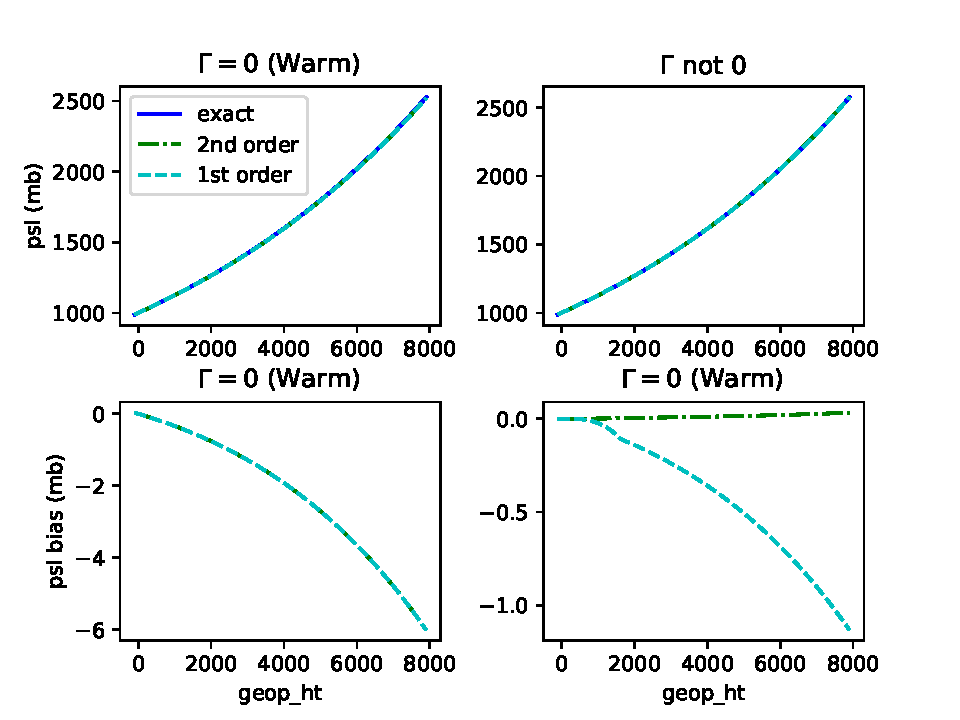
\includegraphics[keepaspectratio=true, width = 4.5in]
{psl_exactVSapprox.pdf}}
\caption{Tests of exact versus approximate $p_s$ calculations. Left panels are warm enough that $\Gamma=0$ ($T_g=292$ K) while right panels use $\Gamma=6.5$ K km$^{-1}$ ($T_g=280$ K). Top panels show actual $p_s$ and bottom panels show bias. Sea level pressures are much too high because $p_g=1000$ mb, but this should be fine for testing purposes. Note that the lowest elevation sampled is -100 m to test behavior when terrain is below sea level.} 
\label{fig:exactVSapprox}
%EXPLANATION:
%/g/g11/caldwep/py/scream/v1/calc_psl.py
\end{figure}
%----------------------------------------------

Fig. \ref{fig:psl_vs_v0} compares $p_s$ from an old F90 simulation against values calculated using our approximate formula. As expected, results look very similar despite using midpoint $T$ as an approximation for $T_g$. Using a first-order rather than 2nd order Taylor series once again has an insignificant effect. 
%----------------------------------------------
\begin{figure}[ht]
\noindent
\centering
\rotatebox{0}{
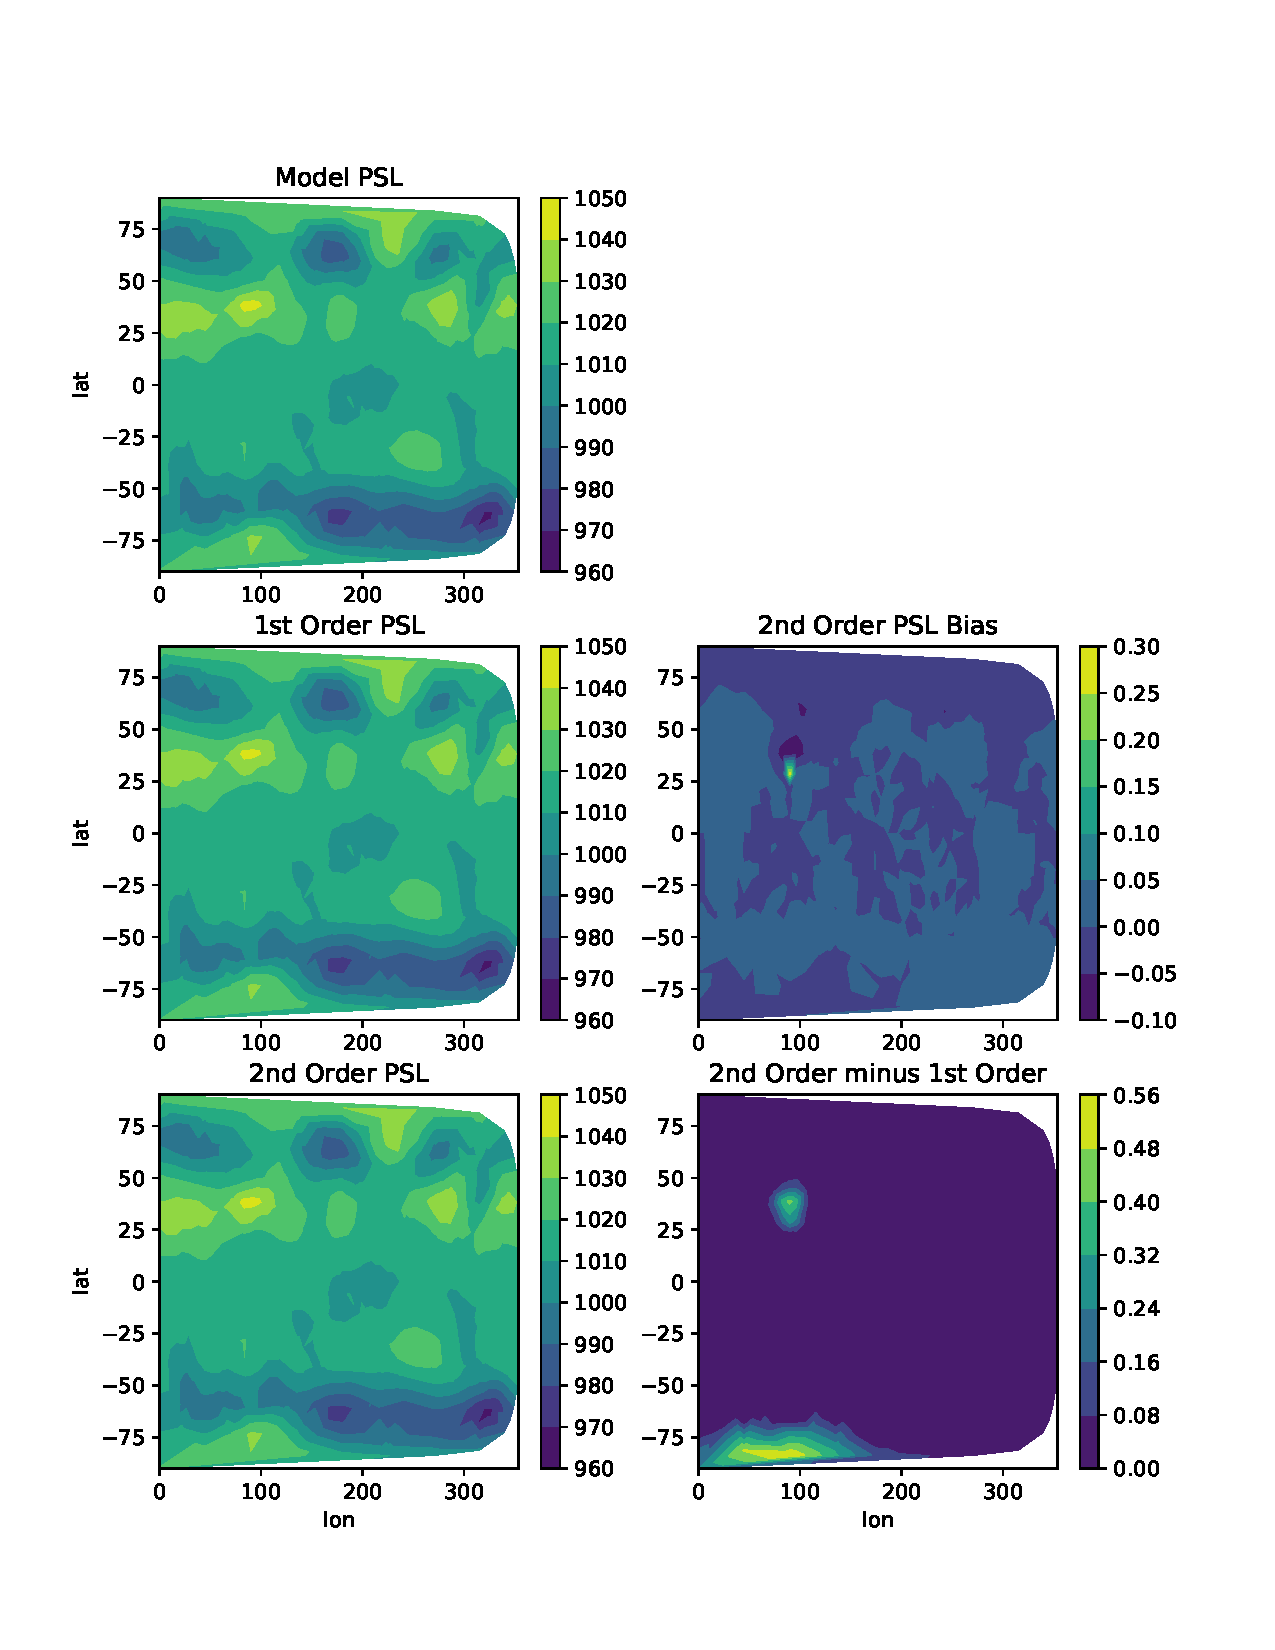
\includegraphics[keepaspectratio=true, width = 5in]
{psl_vs_v0.pdf}}
\caption{Comparison of $p_s$ from an old ne4 F90 model simulation (top left) versus calculation of the same quantity using (\ref{eq:approx_soln}). Panels on the left show $p_s$ and right-hand panels show differences between simulations. Calculated $p_s$ used midpoint rather than surface temperature because the latter wasn't available; this likely accounts for most of the F90 vs new calculation differences we see; despite this imperfection, biases are still acceptably low.} 
\label{fig:psl_vs_v0}
%EXPLANATION:
%/g/g11/caldwep/py/scream/v1/calc_psl.py
\end{figure}
%----------------------------------------------

%================================
\subsection{Unit Tests}
%================================

\begin{enumerate}
\item Is C++ value close to exact solution for very warm conditions where $\Gamma$ should be zero? 
\item Is C++ value close to exact solution for normal conditions where $\Gamma$ should be 6.5 K km$^{-1}$?
\item Is $p_s<p_g$ when $\Phi_ground>0$ (for very cold, moderate, and very warm $T_g$ and a variety of $p_g$ values)?
\item Is $p_s>p_g$ when $\Phi_ground<0$ (for very cold, moderate, and very warm $T_g$ and a variety of $p_g$ values)?
\item Test that modified $T_g$ values for very cold and very warm conditions are applied correctly. Not sure how to do this - should computation of $\widetilde{T_g}$ be its own unit? Or should modified $T_g$ be computed in the unit test itself and stuffed into the exact solution to provide an independent calculation of the expected solution? Or is this too dumb to test?
\end{enumerate}

\bibliography{biblio.bib}




%================================
\section{Bibliography}
%================================
\bibliography{biblio.bib}

\end{document}
